%! Licence = CC BY-NC-SA 4.0

%! Author = gianfluetsch
%! Date = 30. Dez 2021
%! Project = cydef_summary

\section{Forensic Readiness}
Unter Forensic Readiness versteht man die technische und organisatorische Vorbereitung, um im Fall eines Sicherheitsvorfalls schnell und zielgerichtet reagieren und eine IT-forensische Nachuntersuchung optimal durchführen zu können.

\subsection{Forensic Readiness Analyse}
Es sollte eine genaue IST-Analyse der IT-Landschaft durchgeführt, alle bestehenden Richtlinien überprüft und die relevanten Prozesse für den Umgang mit IT-Sicherheitsverletzungen erstellt/ überprüft werden.
So kann ermittelt werden, ob die bestehenden organisatorischen und technischen Strukturen eine adäquate Reaktion auf sicherheitsrelevante Ereignisse zulassen.\\

\begin{itemize}
    \item Welche potentiellen Angriffsszenarien sind relevant (Threat Model)?
    \item Welche Daten müssen im Notfall verfügbar sein?
    \item Wie sehen die optimalen organisatorischen Voraussetzungen dafür aus?
    \item Wie sehen die optimalen technischen Voraussetzungen dafür aus?
\end{itemize}

\subsubsection{Forensic Readiness Optimierung}
Auf Basis der Analyse können wirkungsvolle Maßnahmen, um sowohl die organisatorischen als auch die technischen Voraussetzungen zu optimieren, erarbeitet werden.
Dazu gehört die Umsetzung der Maßnahmen, das erstellen von Checklisten und z.B. auch die entsprechende Schulung der Mitarbeiter.\\

\begin{itemize}
    \item Integration von forensischen Datensicherungen in den Incident Response Prozesse
    \item IT-Richtlinien, die für die Forensic Readiness von Relevanz sind
    \item Umsetzung der Massnahmen
    \item Erstellen von Checklisten
    \item Notwendige Vereinbarungen mit IT-Dienstleistern
    \item Schulung der Mitarbeiter
\end{itemize}

\subsection{Web Forensic Readiness}

\subsubsection{Topologie}
Client $\rightarrow$ WAF $\rightarrow$ APP $\rightarrow$ API $\rightarrow$ DB

\begin{center}
    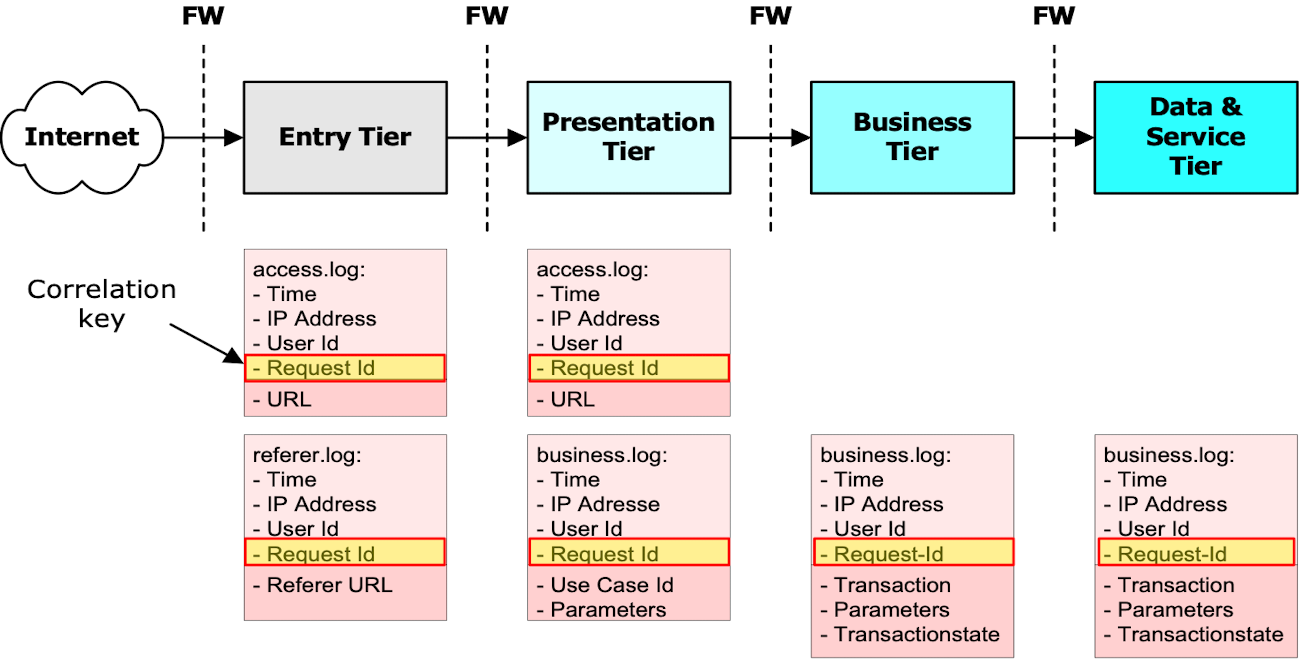
\includegraphics[width=1.0\linewidth]{web_fr}
    \vspace{-8pt}
\end{center}

\subsubsection{Ablauf Request}
\begin{enumerate}
    \item Request zu WAF $\rightarrow$ \textit{Unique\_ID} wird generiert und an Request \glqq angehängt\grqq
    \item Request weiter an APP mit \textit{Unique\_ID} (APP muss diese ID loggen)
    \item Request weiter zu API mit \textit{Unique\_ID} (API muss diese auch loggen)
    \item Request weiter zu DB mit \textit{Unique\_ID} (DB muss diese auch loggen)\\
\end{enumerate}

\textbf{Damit kann über die geloggte \textit{Unique\_ID} nachträglich der Weg jedes Requests herausgefunden und analysiert werden.}

\subsubsection{Unique-ID zum Logfile hinzufügen}
2 verschiedene Arten möglich:
\begin{itemize}
    \item Vorkonfigurierte Protokollrichtlinie ,,ForensicLog`` verwenden (nicht konfigurierbar)
    \item Hinzufügen einer UNIQUE-ID zum benutzerdefinierten Protokoll (sehr flexibel)
\end{itemize}

\subsubsection{Unique-ID Vorteile}
\begin{itemize}
    \item Korrelation von Ereignissen zwischen Multi-Tier- und Mikro-Service-Architekturen
    \item Weil ein Zeitstempel nicht ausreicht
    \item Der erste Server (der dem Internet zugewandt ist) sollte die Unique-ID generieren und sie in die eigenen Protokolldateien aufnehmen. Außerdem sollte die Unique-ID an die Backend-Dienste weitergegeben werden, in der Regel durch Hinzufügen eines speziellen Headers. Die Backend-Dienste sollten die Unique-ID parsen und zu den eigenen Protokollen hinzufügen. Außerdem sollte er die Unique-ID jedem weiteren Server oder jeder weiteren Instanz hinzufügen. Wenn dies bei allen Diensten der Fall wäre, könnten Sie jederzeit herausfinden, wer, wann, wo etwas passiert ist.
    \item Ohne die Unique-ID sind Unternehmen aufgeschmissen und müssen sich auf Zeitstempel verlassen.
\end{itemize}

\newpage

\subsection{MitM}

\subsubsection{Unverschlüsselte Kommunikation}
\begin{enumerate}
    \item Lesen aller Daten (PW, Kreditkarte, Mail)
    \item Manipulieren aller Daten
    \item Drop (DoS)\\
\end{enumerate}

\textbf{Strategien}:
\begin{itemize}
    \item On the fly
    \item Redirect to malicious service
\end{itemize}

\subsubsection{Verschlüsselte Kommunikation}
\begin{enumerate}
    \item Terminate Service (Interception) $\rightarrow$ \textit{CertWarning}
    \item Downgrade (HTTPS $\rightarrow$ HTTP/ TLS Version Downgrade)
    \item Mit unverschlüsseltem Content den verschlüsselten Schwächen
    \item Replay Angriffe
    \item DoS
\end{enumerate}

\subsection{Forensic Readiness Apache Reverse Proxy}
Distributed systems, and those using microservices architectures in particular, scatter the order's log messages further, across multiple locations, to be gathered by centralised logging tools. To make it straightforward to investigate problems, you need a way to group the log messages that relate to a particular order, in all of your systems or services.

\subsubsection{Unique-ID}
Correlation IDs provide the standard solution to this problem. A correlation ID uniquely identifies each \glqq customer order\grqq, or the equivalent in your system. Similarly, web-based applications have \glqq user requests\grqq, for each user interaction

\subsubsection{How do you enable the unique-id in the apache?}
By using the \lstinline|mod_unique_id| module.

\subsubsection{How do you log the unique-id into the forensic log}
\lstinline|mod_log_forensic| is included in most distribution packages of Apache and comes with the source tarball download, but if you compile Apache 2.x.x from source, you need to add \lstinline|--enable-log-forensic| and \lstinline|--enable-unique-id| to the configure line.

\subsubsection{How do you inject the unique-id to the backend service?}
By adding the \textit{UNIQUE\_ID} into the following Request Header towards to backend service. On both parts it will be logged for logs/ time correlation.

\newpage

\subsection{HTTP and HTTPS MitM Apache Reverse Proxy}
This exercise is explaining the so-called online phishing attack. We want to learn how to setup http/https listener, that is forwarding everything to the target webserver. We want to create a \textit{http} and \textit{https} listener and both shall forward to the backend system.
The reverse proxy can be used to forward all traffic to another apache instance within the same docker container.

\subsubsection{Explain the benefit of having a http to https reverse proxy in a phishing campaign}
By using a http to https proxy you ensure having a secured tls connection to the outer world. Having a proxy with unique logging IDs enables for a better traceability for connections especially in a phishing campaign.

\subsubsection{Explain the benefit of having a https to https reverse proxy in a phishing campaign}
By having a https to https proxy as a man-in-the-middle which breaks up tls connections it is able to track connections and its contents for malware/ content filtering and logging with unique IDs. As https reverse proxy internal tls connections are secured by a valid (AD-CA or self-signed distributed) certificate.

\subsubsection{Explain how your reverse proxy online phishing could be advertised to a victim within the same network (LAN)}
With DNS/ ARP spoofing, IPV6 Router Advertisements or Neighbour Discovery fakes.

\subsubsection{Explain how your reverse proxy online phishing could be advertised to a victim over the internet}
With Routing malfunctioning, Domain takeovers, unsecured public DNS. A good mitigation against these attacks is \textit{DNSSec}.

\subsection{Man in the Middle - SSH}
The Man-in-the-Middle (MitM) attack is a cyberattack where the attacker secretly relays and possibly alters the communications between two parties who believe that they are directly communicating with each other. This theory is discussing MitM for the ssh protocol.

\subsubsection{Explain why public/ key auth is really preventing MitM}

\begin{enumerate}
    \item When logging onto the client via ssh on port 4444, it is being forwarded as configured to the ssh server.
    \item The username/pw is being forwarded to the ssh server.
    \item There are no secrets exchanged doing initialization. As the public key is stored on the device, the user is \glqq known\grqq.
    \item The server sends a challenge to the initiating client, the client signs the nonce with the private key and returns it
    to the ssh destination. Identity is proven by this.
\end{enumerate}

\subsubsection{Explain the purpose of editing the ssh client configuration}
The user is identified on the target system by the public key id. The identity is validated by the correct signature of the nonce by the client sent to the server back. Only possible with the correct private key.

\subsubsection{Explain why 2FA would not fix the problem of ssh MitM}
\begin{itemize}
    \item 2FA doesn't help if the purpose are live (on the fly).
    \item If a attacker claims to have the private key and a 2FA message is sent to the (correct) owners smartphone, it does help, as the user wouldn't confirm the request.
\end{itemize}

